\begin{figure}[ht]
\begin{center}
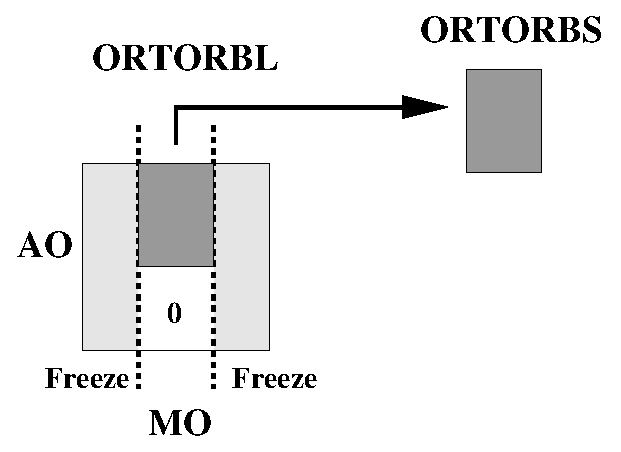
\includegraphics[width=7cm,keepaspectratio]{02_localization/images/matrix.eps}
\caption{\footnotesize A visual representation of large (ORTORBL) and small (ORTORBS)
molecular orbitals matrices. Localized orbitals are first classified as frozen or
non-frozen. The non-frozen orbitals are supposed to have negligible
coefficients on distant atoms. These coefficients are strictly set to
zero by the cut procedure, and a localized optimization is performed in the
obtained AO/MO subspace. }
\label{fig:matrix}
\end{center}
\end{figure}

